\begin{center}



\tikzset{every picture/.style={line width=0.75pt}} %set default line width to 0.75pt        

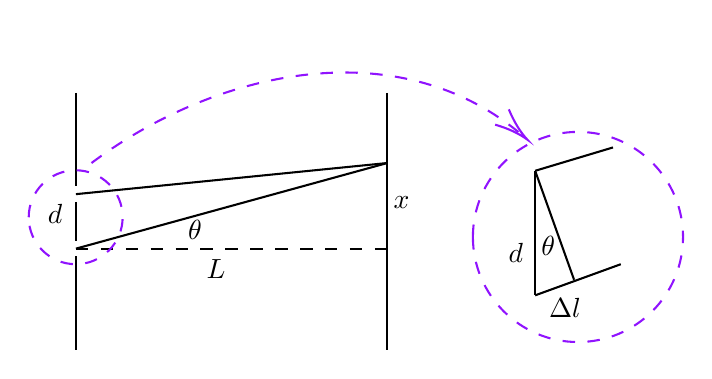
\begin{tikzpicture}[x=0.75pt,y=0.75pt,yscale=-1.5,xscale=1.5]
%uncomment if require: \path (0,300); %set diagram left start at 0, and has height of 300

%Straight Lines [id:da7937139484326525] 
\draw    (130,55) -- (130,85) ;
%Straight Lines [id:da5514747070310864] 
\draw    (130,90) -- (130,102.5) ;
%Straight Lines [id:da3180465848105889] 
\draw    (130,107.5) -- (130,137.5) ;
%Straight Lines [id:da26896276424224896] 
\draw    (230,55) -- (230,137.5) ;
%Straight Lines [id:da7167210011053942] 
\draw  [dash pattern={on 4.5pt off 4.5pt}]  (130,105) -- (230,105) ;
%Straight Lines [id:da7138419970578529] 
\draw    (130,105) -- (230,77.5) ;
%Straight Lines [id:da7800441168755299] 
\draw    (130,87.5) -- (230,77.5) ;
%Shape: Circle [id:dp49969692270722277] 
\draw  [color={rgb, 255:red, 144; green, 19; blue, 254 }  ,draw opacity=1 ][dash pattern={on 4.5pt off 4.5pt}] (114.83,94.92) .. controls (114.83,86.58) and (121.58,79.83) .. (129.92,79.83) .. controls (138.25,79.83) and (145,86.58) .. (145,94.92) .. controls (145,103.25) and (138.25,110) .. (129.92,110) .. controls (121.58,110) and (114.83,103.25) .. (114.83,94.92) -- cycle ;
%Curve Lines [id:da6541923848279152] 
\draw [color={rgb, 255:red, 144; green, 19; blue, 254 }  ,draw opacity=1 ] [dash pattern={on 4.5pt off 4.5pt}]  (135,77.5) .. controls (174.6,47.8) and (233.56,34.36) .. (273.79,68.94) ;
\draw [shift={(275,70)}, rotate = 221.74] [color={rgb, 255:red, 144; green, 19; blue, 254 }  ,draw opacity=1 ][line width=0.75]    (10.93,-3.29) .. controls (6.95,-1.4) and (3.31,-0.3) .. (0,0) .. controls (3.31,0.3) and (6.95,1.4) .. (10.93,3.29)   ;
%Straight Lines [id:da18744774929107222] 
\draw    (277.5,80) -- (302.5,72.5) ;
%Straight Lines [id:da2397390109705031] 
\draw    (277.5,120) -- (305,110) ;
%Straight Lines [id:da21304007677005732] 
\draw    (277.5,80) -- (277.5,120) ;
%Straight Lines [id:da6975177627780123] 
\draw    (277.5,80) -- (290,115) ;
%Shape: Circle [id:dp9982306358023718] 
\draw  [color={rgb, 255:red, 144; green, 19; blue, 254 }  ,draw opacity=1 ][dash pattern={on 4.5pt off 4.5pt}] (257.5,101.25) .. controls (257.5,82.61) and (272.61,67.5) .. (291.25,67.5) .. controls (309.89,67.5) and (325,82.61) .. (325,101.25) .. controls (325,119.89) and (309.89,135) .. (291.25,135) .. controls (272.61,135) and (257.5,119.89) .. (257.5,101.25) -- cycle ;

% Text Node
\draw (171,107.4) node [anchor=north west][inner sep=0.75pt]  [font=\normalsize]  {$L$};
% Text Node
\draw (120,89.9) node [anchor=north west][inner sep=0.75pt]  [font=\normalsize]  {$d$};
% Text Node
\draw (231,87.4) node [anchor=north west][inner sep=0.75pt]  [font=\normalsize]  {$x$};
% Text Node
\draw (268,102.4) node [anchor=north west][inner sep=0.75pt]  [font=\normalsize]  {$d$};
% Text Node
\draw (165,95) node [anchor=north west][inner sep=0.75pt]  [font=\normalsize]  {$\theta $};
% Text Node
\draw (278.5,100) node [anchor=north west][inner sep=0.75pt]  [font=\normalsize]  {$\theta $};
% Text Node
\draw (281,119.9) node [anchor=north west][inner sep=0.75pt]  [font=\normalsize]  {$\Delta l$};


\end{tikzpicture}

\end{center}